\documentclass[12pt,fleqn]{article}\usepackage{../../common}
\begin{document}
Ders 6

Bu derste işlenecek önemli konular şunlar, bir matrisin kolon uzayı
(columnspace), ki bu konuya önceki derste değindik, diğeri ise bir
matrisin sıfır uzayı (nullspace) ve alt uzaylar. 

Şimdi alt uzaylar hakkında bir düşünce deneyi yapalım. Diyelim ki elimde $P$
ve $L$ diye iki tane alt uzay var, $P$, $\mathbb{R}^3$ içinde bir düzlem
(plane), $L$ ise $P$ üzerinde olmayan bir çizgi (line). $P$ ve $L$ tabii ki
orijinden geçiyorlar, yoksa alt uzay olmazlar. 

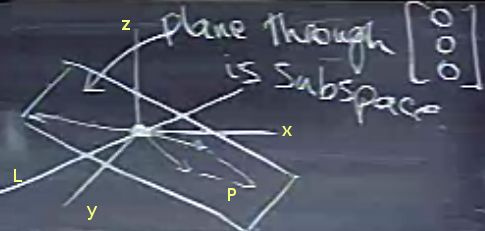
\includegraphics[height=4cm]{6_01.png}

[Üstteki resimdeki yazı orijinden geçen düzlem altuzaydır diyor]. Soru şudur; bu
iki uzayın birleşimi (union) bir alt uzay oluşturur mu?  Cevap hayır. Çünkü
belirtilen müstakbel uzay toplanabilme prensibine izin vermiyor. Bu prensibe
göre bir uzay içindeki iki vektörün toplamı aynı uzay içinde olmalıydı değil mi?
Bir çizgi ve düzlemin toplamı olan ``şey'' bu tanıma uymuyor. Gayet rahat bir
şekilde düzlemden bir vektör, $L$'den bir vektör alıp onları toplarsam bambaşka
bir yöne işaret eden bir yeni vektör elde edebilirim ve bu vektör $P \cup L$
içinde olmaz.

Peki $P \cap L$'i düşünelim, yani her iki uzayın kesişimi olan küme bir
alt uzayı mıdır? Kesişimde ne olduğunu düşünelim, sadece orijin noktası
var, o zaman kümede sadece sıfır noktası var. Sıfır vektörü tek başına bir
alt uzay oluşturabilir mi? Evet. Bu küme bir alt uzay oluşturabilir mi?
Cevap yine evet. 

Soruyu daha genelleştirerek soralım: herhangi iki alt uzay $S,T$'yi alalım,
$S \cap T$ her zaman bir alt uzay olur mu? Bu alt uzay daha ufak olacaktır,
çünkü şartları daha spesifik hale getirdik, bir nokta hem $S$ hem $T$
içinde olmalıdır, herhalde bu şarta uyan noktalar daha azdır. Ama cevap
yine evet. Düşünelim; kesişimden $v,w$ adlı iki vektör alalım, o zaman $u +
w$, $S$ içinde mi? Evet, çünkü $u,w$'nin ikisi de tanım itibariyle $S$
içinde, ve $S$ bir alt uzay olduğuna göre onun içindeki iki vektörün
toplamı da aynı uzay içinde olmlaya meburdur, ve aynı durum $T$ için de
geçerlidir. Toplam demek ki hem $S$ hem $T$ içinde olacaktır, bunu
söylerken yani ``hem $S$ hem $T$ içinde'' derken aynı zamanda kesişimi
tarif etmiş olmadık mı? Evet, o zaman toplam aynı zamanda kesişim içindedir
de. İspat tamamlandı.

Alt uzay kontrolünün ikinci öğesi neydi? Sabitle çarpım yine uzay içinde
olmalı. Aynı argümanı kullanıyoruz, $S \cap T$ içinde olan bir vektörü
alırım, mesela 7 ile çarparım, sonuç yine $S$ içinde çünkü $S$ bir alt
uzaydı, $T$ içinde, aynı sebepten dolayı. Demek ki çarpım hem $S$ hem $T$
içinde bu sebeple $S \cap T$ içinde.

O zaman iki alt uzayın kesişimi kesinlikle bir alt uzaydır. 

$A$'nin Kolon Uzayı

$$ A = 
\left[\begin{array}{rrr}
1 & 1 & 2 \\
2 & 1 & 3 \\
3 & 1 & 4 \\
4 & 1 & 5 
\end{array}\right]
 $$

Bu matrisin kolon uzayı $\mathbb{R}^4$'un bir alt uzayıdır çünkü kolondaki
vektörler 4 boyutlu. $A$'nin kolon uzayında, ki buna $C(A)$ diyelim, ne
vardır? Üstte gördüğümüz $A$'nin tüm kolonları, üçü de, oradadır. Ama bu
yeterli değil tabii ki, değil mi? 3 tane vektör koyarak bir alt uzay elde
etmiş olmam. Bu alt uzayı nasıl doldururum? Üstteki üç vektörün tüm lineer
kombinasyonlarını alırım ve alt uzaya koyarım. Bunu yaparsam bir vektör
uzayı elde etmiş olabilirim fakat hala bir alt uzay elde etmiş olmam. 

Üstteki üç vektörün tüm kombinasyonları tüm 4 boyutlu uzayı (yani
$\mathbb{R}^4$) doldurur mu? Cevap hayır. Yani ispatsal olarak bunu
göstermemiş olsak bile sezgimiz bunun olmayacağı yönünde (ki bu sezgi
doğru). 

Fakat bu kombinasyonlar daha ufak bir uzay olacağı kesin. Ne kadar ufak? 

Bu sorunun cevabını vermek için lineer denklemler ile bir bağlantı kurmak
faydalı olacak. Sorular şunlar,

``$Ax = b$ denkleminin her $b$ için bir çözümü var mıdır?''

Bir diğer bağlantılı soru, ``hangi $b$'ler için çözüm vardır?''

1'inci sorunun cevabı hayır; çünkü elimde 4 tane denklem, ama 3 tane
bilinmeyen var, yani bazı $b$'ler için çözümün olmaması gayet
normal. Üstteki örneği genişletirsek,

$$ A = 
\left[\begin{array}{rrr}
1 & 1 & 2 \\
2 & 1 & 3 \\
3 & 1 & 4 \\
4 & 1 & 5 
\end{array}\right]
\left[\begin{array}{r}
x_1  \\
x_2  \\
x_3  
\end{array}\right] 
=
\left[\begin{array}{r}
b_1  \\
b_2  \\
b_3  \\
b_4  
\end{array}\right]
 $$

Fakat ``bazı'' (eşitliğin) sağ tarafları için bu denklemin çözümü
vardır. Bu da 2. sorunun cevabını verecek, ilgilendiğim sağ taraflar
bunlar. 

En bariz $b$ hangisi? Sıfır vektör. O zaman $x$'i de sıfır vektör alırım,
ve bu bir çözüm olur. Bir diğer çözüm? [Sınıftan bir cevap geliyor, hoca
yazıyor]


$$ A = 
\left[\begin{array}{rrr}
1 & 1 & 2 \\
2 & 1 & 3 \\
3 & 1 & 4 \\
4 & 1 & 5 
\end{array}\right]
\left[\begin{array}{r}
x_1  \\
x_2  \\
x_3  
\end{array}\right] 
=
\left[\begin{array}{r}
1  \\
2  \\
3  \\
4  
\end{array}\right]
 $$

Bu $b$ için çözüm vardır? Hangi $x$ bu denklemi çözer? Haldir huldür hücre
hücre çarpımı yapmaya gerek yok. Çarpıma kolon bakışını kullanırsak, çözüm
basit, zaten $b$, $A$'nin birinci kolonu ile aynı. O zaman 1. kolondan 1
tane, 2. ve 3. kolondan 0 tane almak bize çözümü verir, yani

$$ A = 
\left[\begin{array}{rrr}
1 & 1 & 2 \\
2 & 1 & 3 \\
3 & 1 & 4 \\
4 & 1 & 5 
\end{array}\right]
\left[\begin{array}{r}
1  \\
0  \\
0  
\end{array}\right] 
=
\left[\begin{array}{r}
1  \\
2  \\
3  \\
4  
\end{array}\right]
 $$


Bir başka çözüm, mesela $A$'nin ikinci kolonu $b$ olsaydı, o zaman 
$x = \left[\begin{array}{rrr} 0 & 1 & 0 \end{array}\right]^T$ bir çözümdür,
vs.. Tabii $b$ bulmanın daha basit yolu, herhangi bir $x$ seçerim, çarpımı
yaparım, $b$ elde ederim. Bunu yaparken $A$'nin kolonlarının lineer
kombinasyonlarını almış olmuyor muyum? Evet. Ve nihayet 2. sorunun cevabına 
geldik; $Ax=b$'yi sadece eğer $b$, $A$'nin kolon uzayında ise çözebilirim. 

Niye olduğunun üzerinden bir daha geçelim. $A$'nin kolon uzayı tanım
itibariyle tüm mümkün $Ax$'leri taşımak mecburiyetindedir, yani mümkün tüm
$x$'ler $A$'yi çarpar, yani ``onun kolonlarını kombine eder'', ve bu kolon
uzayını oluşturur. 

Şimdi kolon uzaylarıyla yakından alakalı yeni bir soru daha soralım;
$A$'nin tüm kolonları birbirinden bağımsız midir (independent)? Yani
$A$'nin her kolonu kolon uzayına ``yeni bir şeyler ekler mi?''. Bu ifadeyle
şunu kastediyoruz, eğer 3. kolon 1. ve 2.'nin kombinasyonu ise, 3. kolon
uzaya bir yenilik katmıyor demektir, çünkü 3. kolonu kullanmak yerine 1. ve
2.'yi kullanmak yeterli olacaktır. 

$A$'ya dikkatle bakalım, $A$'nin herhangi bir kolonunu atsak, yine aynı
kolon uzayını elde eder miyiz? $A$'nin bağımsız olmayan, diğerlerinin
kombinasyonu olan kolonu var mıdır? Evet. 

$$ A = 
\left[\begin{array}{rrr}
1 & 1 & 2 \\
2 & 1 & 3 \\
3 & 1 & 4 \\
4 & 1 & 5 
\end{array}\right]
 $$

3'üncü kolon bariz bir şekilde 1. ve 2.'nin toplamı. Demek ki 1. ve 2. kolon
$A$'nin pivot kolonları, 3. değil. Fakat bir dakika, 3. kolonu kötü çocuk
ilan etmeden, bakalım acaba 1. kolonu atsak, yine aynı kolon uzayını elde
eder miydik? Cevap yine evet, çünkü 1. kolon 3.'nun 2.'den çıkartılmış hali
de denebilir! O zaman 1. kolon atılıp 2. ve 3. bağımsız olarak
tutulabilirdi. Fakat ben prensip / alışkanlık bağlamında  soldan
sağa giderim, bağımsızlığı solda ilk baktığım kolonlara göre
irdelemeye uğraşırım.

Sonuç olarak, $A$'nin kolon uzayı $\mathbb{R}^4$'un iki boyutlu bir alt
uzayıdır. İki boyutlu çünkü bağımsız sadece iki kolon (vektör) var, bu iki
vektör sadece bir iki boyutlu düzlemi (plane) tanımlayabilir. 

Sıfır Uzayı

Tamamen farklı türde bir vektör /alt uzaydan bahsetmek istiyorum şimdi; sıfır
uzayı. Mesela $A$'nin sıfır uzayında ne vardır? 

Bu uzayda $A$'nin kolon kombinasyonları yoktur. Farklı bir şekilde, $Ax$
denklemi bağlamında, $x$'ler vardır. Hangi $x$'ler? $Ax=0$ denkleminin çözüm
olabilecek tüm $x$'ler. Yani,

$$ A = 
\left[\begin{array}{rrr}
1 & 1 & 2 \\
2 & 1 & 3 \\
3 & 1 & 4 \\
4 & 1 & 5 
\end{array}\right]
\left[\begin{array}{r}
x_1  \\
x_2  \\
x_3  
\end{array}\right] 
=
\left[\begin{array}{r}
0  \\
0  \\
0  \\
0  
\end{array}\right]
 $$

$x$'lerin 3 öğesi var, o zaman $A$'nin sıfır uzayı $\mathbb{R}^3$'un bir
alt uzayı (tabii önce bu uzayın düzgün bir alt uzay olduğunu da
ispatlamamız gerekir, ve bunu göstereceğiz). 

$A$'ya çıplak gözle bakarak bu sıfır uzayını bulabilir miyiz? Her veri
üzerinde işleyecek teknik tabii ki eliminasyon yapmak, vs. ve sonucu böyle
bulmak. Fakat bu basit örnek üzerinde sonucu hemen bulabilir miyiz? 

İlk çözüm, $x=0$. Bu bariz olan ilk çözüm. Sıfır uzayında sıfır vektörü
var, ki sıfır uzayı bir vektör uzayı olma şansı artmış oldu böylece (çünkü
tüm vektör uzaylarında sıfır vektörü olmalı). 

Bir diğer çözüm? Aradığım $A$'nin kolon kombinasyonları, öyle ki o
kombinasyon sıfır vektörü olsun. Bir tanesi,

$$ A = 
\left[\begin{array}{rrr}
1 & 1 & 2 \\
2 & 1 & 3 \\
3 & 1 & 4 \\
4 & 1 & 5 
\end{array}\right]
\left[\begin{array}{r}
1  \\
1  \\
-1  
\end{array}\right] 
=
\left[\begin{array}{r}
0  \\
0  \\
0  \\
0  
\end{array}\right]
 $$

Bir başkası? $\left[\begin{array}{rrr}2 & 2 & -2\end{array}\right]^T$,
yani bir önceki çözümün iki katı. Bir kalıp ortaya çıkmaya başladı; Tüm
çözümler neye benzer? $c \cdot \left[\begin{array}{rrr}1 & 1 &
-1\end{array}\right]^T$, ki sabit $c=7$, olabilir, $c=11$
olabilir.. Tüm bu sıfır uzayının çizsem neye benzer? Bir çizgi olmaz mı?
Evet. Bu çizgi de sıfırdan geçer zaten,

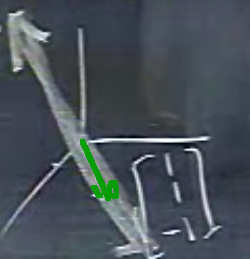
\includegraphics[height=4cm]{6_02.png}

[Yeşil ok $\left[\begin{array}{rrr}1 & 1 & -1\end{array}\right]^T$ ve tüm
çizgi onun katları]. Yani sıfır uzayı $\mathbb{R}^3$'de bir çizgidir. 

Peki bu sıfır uzayı bir alt uzay midir? Bir uzaya ``uzay'' demek sadece
onun belli şartlara uyması ile mümkündür. Bu şartlar var mı ona bakalım.

$Av=0$ ise ve $Aw=0$ ise, o zaman $A(v+w)=0$ olmalı, yani $v$ sıfır
uzayında ise, $w$ sıfır uzayında ise, $v+w$ de sıfır uzayında olmalı. İspat
son derece basit, 

$$ A(v+w) = 0 $$

$$ Av + Aw = 0 $$

ki $Av=0$ ve $Aw=0$ olduğunu biliyorum, o zaman 

$$ \cancelto{0}{Av} + \cancelto{0}{Aw} = 0 + 0 = 0 $$

Bu ispat tamam. Şimdi 2. kontrol; sabitle çarpım sıfır uzayında mıdır? 

$$ Ax = 0  $$

$$ A(c \cdot x) = 0  = c \cdot Ax = 0 = c \cdot \cancelto{0}{Ax} = 0$$

Bu şart da yerine getirildi. 

Şimdi, karşılaştırma amaçlı olarak, sıfır uzayı olmayan bir örneğe bakalım,

$$ A = 
\left[\begin{array}{rrr}
1 & 1 & 2 \\
2 & 1 & 3 \\
3 & 1 & 4 \\
4 & 1 & 5 
\end{array}\right]
\left[\begin{array}{r}
x_1  \\
x_2  \\
x_3  
\end{array}\right] 
=
\left[\begin{array}{r}
1  \\
2  \\
3  \\
4  
\end{array}\right]
 $$

Bunu çözen $x$'ler bir vektör uzayı oluştururlar mı? Cevap hayır. Bunu
görmenin en basit yolu, sıfır vektörünün çözüm olmadığının
görmektir. Sıfır vektörü yoksa orijin yok demektir, orijin yoksa bir uzay
elde edemeyiz. 

Bir çözüme bakalım, $x = \left[\begin{array}{rrr} 1&0&0 \end{array}\right]^T$. 
Diğeri?  $x = \left[\begin{array}{rrr} 0&-1&1 \end{array}\right]^T$

Böyle bir sürü çözüm var, fakat bunlar bir alt uzay değil.. Büyük bir
ihtimalle bu çözümler bir çizgi ya da düzlem oluşturuyorlar, ama orijinden 
geçmiyorlar. 


\end{document}
